\documentclass{article}
\usepackage{listings}
\usepackage{graphicx}
\usepackage{hyperref}
\usepackage{xcolor}
\usepackage{sidecap}
\usepackage[utf8]{inputenc}

\graphicspath{ {./images/} }
\hypersetup{pdfborder=0 0 0}

\begin{document}
    
    \begin{titlepage}
        \begin{center}
            \hspace{0cm}
            \vfill
            
            \Huge
            CT Projekt: Boids
            
            \vspace{0.3cm}
            
            \Large
            Schwarmsimulation mit SFML Graphic Library in C++
            
            \vspace{0.3cm}
            
            \large
            Gabriel Kraus und Alexander Klee
            
            \vspace{0.3cm}
            
            20.10.2021 - 11.01.2022
            
            \vfill
            \hspace{0cm}
        \end{center}
    \end{titlepage}

    \tableofcontents
    \pagebreak
    
    \section{Projektbeschreibung}
    In der Projektplanungsphase haben wir uns dazu entschieden “Boids” zu simulieren. Nach einiger Überlegung entschieden wir uns für die Programmiersprache C++. Diese ist für Graphikanwendungen zwar eher weniger bekannt und schwieriger zu nutzen, jedoch ist sie sehr gut geeignet für aufwändige berechnungen. Das kann wichtig werden, wenn man eine sehr große Anzahl an Boid-Objekten Simuliert, da die Rechenzeit pro Boid exponentiell steigt. 
    \newline
    Boids sind eine Simulation von künstlichem Leben und folgen 3 Regeln:
    \begin{itemize}
        \item Cohesion - Zusammenhang, von Boids 
        \item Separation - Separation, von anderen Boids 
        \item Alignment - Angleichung, der Bewegungsrichtung der anderen Boids
    \end{itemize}
    Dabei entsteht eine Art Muster aus dem Chaos, der zufällig erzeugten Boids. Sie bilden kleine Gruppen und schwärmen umher. Die Technologie der Boids findet Anwendung in Filmen und Videospiele z.B. Batman Returns, bei dem ein großer Schwarm von Fledermäusen simuliert wird oder Half-Life bei dem Vogelartige Kreaturen dargestellt werden. 
    
    \section{Ziele}
    \subsection{Mindest Ziele}
        Das Ziel des Projektes war eine Simulation der Boids flüssig mit mindestens 100 Objekten zu simulieren, welche sich nach den drei Regeln Separation, Cohesion und Alignment gegenseitig beeinflussen. 
        Zudem war ebenfalls die Idee anhand des Projektes C++ zu lernen und Erfahrung mit der Grafik-Bibliothek SFML sammeln.
    
    \subsection{Weiter Ziele}
        Wenn noch genügend Zeit verbleibt sind weiter Ziele:
        \begin{itemize}
            \item hinzufügen von neuen Boids durch Maus-Inputs
            \item anpassung der drei Parameter Separation, Cohesion und Alignment, sowie der Viewrange der Boids
            \item ‘Feindliche‘ Boids, welche den Rest der Boids jagt
            \item Räumliche Daten Struktur, wie einen Quad Tree, mit welchem die exponentielle Natur der Boids gebändigt werden kann
        \end{itemize}
    
    
    \section{Ergebnisse}
    Dadurch, dass Wir (vor allem Alex) noch C++ lernen mussten und keinerlei Erfahrung mit SFML hatten, ist sehr viel Zeit dabei verbracht worden ein erstes laufendes Beispiel mit SFML zu erstellen. Vor allem das Aufteilen des Programms auf mehrere .cpp Dateien hat leider nicht mit dem Compiler Mingw-32 funktioniert. Um dies trotzdem zu ermöglichen haben wir dann mitten im Projekt die Migration zu Visual Studios, welches automatisch das Makefile richtig erstellt, begonnen. 
    
    Gelungen ist ein Boid-Simulations-Programm, welches anhand von drei anpassbaren Parametern problemlos hunderte, je nach PC sogar tausend Boids und deren Interaktionen Simulieren kann.
    Durch drücken der linken Maustaste werden weitere Boids hinzugefügt, und simuliert.
    Des weiteren ist es möglich die drei Parameter Separation, Cohesion und Alignment während das Programm läuft zu ändern, wobei nach Aktuellem stand das User-Interface, zwar wahrscheinlich bei Minimalisten gut ankommt, für normale Benutzer jedoch weniger als optimal ist.
    \newline Zeit für feindliche Boids oder einer ausgeklügelten Datenstruktur für die Position der Boids hatten wir jedoch leider nicht mehr.
    
    \section{Zusammenarbeit}
    Leider ist es schwierig die genaue Leistung der einzelnen Personen im Nachhinein zu ermitteln, auch deshalb, da ein signifikanter teil der Zeit damit verbracht wurde C++ genauer kennen zu lernen und SFML zum Laufen zu bekommen und sich mit dessen Dokumentation auseinander zu setzten. Das Projekt hat ungefähr eine gesamt Arbeitszeit von 27.5 Stunden, inklusive der Zeit im Unterricht, der Zeit zu Hause alleine und der Zeit in der wir uns im privaten Raum getroffen haben.
    
    \section{Set-Up von SFML}
    Von unserer Erfahrung empfehlen wir die Anleitung von \href{https://www.sfml-dev.org/tutorials/2.5/start-vc.php}{sfml-dev.org}, der offiziellen Website der Graphikbibliothek. Die Anleitung ist für Visual Studio Versionen 2017 und älter, funktioniert jedoch auch problemlos mit neueren Versionen. Es ist auch möglich sich selbst SFML mit CMake zu 'compilieren' und dann mit einem Compiler manuell alles zu linken, jedoch sollte man hierbei sich schon relativ gut mit dem Linker und Compiler auseinander gesetzt haben.
    
    \section{Programm}
        \subsection{Fähigkeiten}
            Nach dem Starten des Programms fängt direkt die Simulation an, werden so viele Boids auf dem Bildschirm zufällig verteilt wie in \textcolor{blue}{main()} angegeben wurden. Jedem dieser Boids wird auch ein zufälliger Gechwindigkeitsvektor zugewiesen, welcher sich jeden Frame nach den drei Regeln neu berechnet. Wenn die Linke Maustaste gedrückt gehalten wird, werden kontinuierlich neue Boids an der Position der Maus erstellt. Mit der Maus lässt sich ebenfalls mithilfe der drei Rechtecke oben links die drei Parameter Separation, Cohesion und Alignment anpassen. Wenn auf das am weitesten links gelegene Rechteck die Rechte Maustaste drückt, nimmt die Separation zu, mit der Linken Taste ab. Die mittlere Box Kontrolliert den Wert Alignment, und die rechte Box die Cohesion.
        
        \subsection{Funktionsweise}
            Die einzelnen Boids bewegen sich nach drei Regeln: Separation, Cohesion und Alignment. Jeden Frame werden diese neu Berechnet. 
            \newline Die Methode \textcolor{blue}{Boid::update\_movement()} Berechnet für jeden dieser Regeln neuen Vektoren  und addiert diesen zu dem Geschwindigkeitsvektor (\textcolor{blue}{Velocity}).
            
            \vspace{0.3cm}
            Somit wird jeden Frame für jeden Boid folgendes berechnet: 
            
            \sidecaptionvpos{figure}{c}
            \begin{SCfigure}[][!ht]
                \centering
                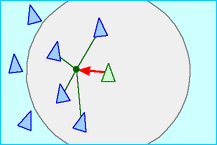
\includegraphics[width=7cm]{images/cohesion.png}
                \caption{Cohesion  Bei der Cohesion wird die Positionen der Boids im Sichtradius summiert und danach durch die Anzahl der Boids geteilt. Davon wird dann die Position des aktuellen Boids abgezogen um die Distanz zu diesem Mittelpunkt zu bekommen.}
            \end{SCfigure}
            
            \begin{SCfigure}[][!ht]
                \centering
                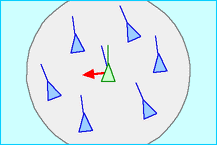
\includegraphics[width=7cm]{images/alignment.png}
                \caption{Alignment Das Alignment ist sehr ähnlich zur Cohesion, allerdings wird die Geschwindigkeit summiert und dann dividiert, um den Durchschnitt der Geschwindigkeit zu bekommen.}
            \end{SCfigure}
            
            \begin{SCfigure}[][!ht]
                \centering
                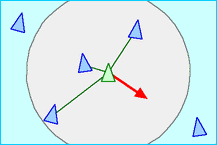
\includegraphics[width=7cm]{images/separation.png}
                \caption{Separation Genauso wie bei Alignment und Cohesion wird bei der Separation ebenfalls ein Vektor aufsummiert, jedoch wird dieses Mal die Distanz summiert und durch die Anzahl dividiert. Dieser Durchschnitt wird später negiert (umgedreht), weil die Separation von den Boids wegzeigen soll, nicht dahin.}
            \end{SCfigure}
        \pagebreak
        
        \subsection{Bugs}
            Während dem Programmieren sind natürlich unzählig viele Bugs aufgetreten, jedoch waren ein paar dieser Bugs besonders interessant oder haben viel Zeit gekostet.
            Ein Beispiel für einen Bug der sogar beides ist, ist ein 'include loop' gewesen. Dadurch, dass die Header-Files in einer Falschen Reihenfolge waren, konnte der Compiler nie zur Definition von \textcolor{blue}{Boid} und \textcolor{blue}{Vector2D} kommen. Ein Temporärer fix war es eine Deklaration (Bsp.: \textcolor{blue}{class Boid;}) ohne Definition von den beiden Klassen in Display.hpp und Boid.hpp zu machen. Inzwischen sind die Header jedoch in der richtigen Reihenfolge, wodurch dies sowieso kein Problem mehr ist. 
            Die am Bugs welche am frustrierendsten waren jedoch die Bugs, welch nicht mal einen Compiler Fehler erzeugt haben. Das kam öfters vor während des implementieren der drei Regeln nach welchen sich die Boids bewegen. Ein Beispiel dafür ist das lange Zeit dieser Algorithmus einfach nicht wirklich wollte - nach langwierigen Debuggen und Loggen von verschiedensten Variablen unter all möglichen Zuständen, stellte sich heraus das die Funktion zum Berechnen der Distanz kompletter Mist war. Wo diese wirklich herkam ist uns immer noch unklar, eine Vermutung ist, dass sie nur halb hingeschrieben und danach einfach vergessen wurde. Nachdem diese Funktion gefixt wurde funktionierte der Algorithmus ohne Probleme.
        
        \subsection{UML diagramm}
            Das UML-Diagramm beinhaltet nur die Klassen die von uns geschrieben worden sind, keine Assoziationen zu Klassen von SFML oder C++.
            
            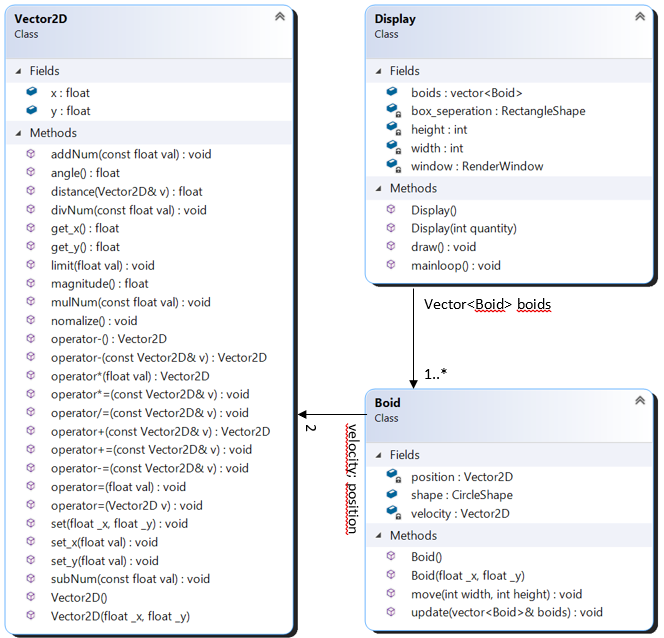
\includegraphics[width=15cm]{images/Class Diagramm.png}
    
    \pagebreak
    
    \section{Quellen}
        \begin{itemize}
            \item http://www.red3d.com/cwr/boids/
            \item https://www.sfml-dev.org/
            \item https://stackoverflow.com/
            \item https://en.cppreference.com/w/
            \item https://www.geeksforgeeks.org/c-plus-plus/
            \item https://en.wikipedia.org/wiki/Boids
            \item https://eater.net/boids
            \item https://cs.stanford.edu/people/eroberts/courses/soco/projects/2008-09/modeling-natural-systems/boids.html
            \item https://github.com/jyanar/Boids/tree/master/
            \item https://www.reddit.com/r/sfml/
            \item https://www.youtube.com/watch?v=QbUPfMXXQIY
            \item https://gamedevelopment.tutsplus.com/tutorials/3-simple-rules-of-flocking-behaviors-alignment-cohesion-and-Separation--gamedev-3444
            \item https://www.youtube.com/watch?v=18c3MTX0PK0\newline\&list=PLlrATfBNZ98dudnM48yfGUldqGD0S4FFb
            \item https://www.youtube.com/watch?v=tYspMwzV8w
        \end{itemize}
        

    
    
\end{document}